\subsection{Problem Statement}

\subsubsection{Determining Data Set}

Data collection will be conducted using the FinanceDataReader package in Python\cite{FinanceDataReader}. 
This package serves as a data crawler, extracting information from Korea Exchange\cite{KRX} for Korean stock data and NASDAQ\cite{NASDAQ} for US stock data. 
It provides access to historical and up-to-date data, making it suitable for both prediction and training/validation/testing purposes.

\subsubsection{Determining Model}

Stock prices exhibit one-dimensional, non-stationary, time-series characteristics. 
In consideration of these unique traits, the selection of an appropriate model is crucial.

\subsubsection{Determining Loss Function and Evaluation Metric}

The choice of a loss function and evaluation metric hinges on the nature of our stock price prediction task. 
If we are predicting only daily price movements (rise/fall), the appropriate loss function will be Cross Entropy, and the evaluation metric will be Accuracy. 
Conversely, if we aim to predict specific values such as closing prices, the preferred loss function will be Huber Loss or Mean Squared Error (MSE), 
and the evaluation metric will be Mean Absolute Error (MAE) or Root Mean Square Error (RMSE).

\subsection{Proposed Solutions}
\subsubsection{LSTM}
Long Short-Term Memory(LSTM) is an advanced Recurrent Neural Network (RNN) architecture 
as shown in the Figure. 
LSTMs were introduced to address some of the limitations of traditional RNNs, 
which struggle with capturing long-range dependencies in sequential data due to the vanishing gradient problem.

LSTM has three gates: input gate, forget gate, and output gate.
\begin{enumerate}
	\item Input gate: 	Input gate is denoted by orange box. It decides what new information should be stored in the cell.
	\item Forget gate:	Forget gate is denoted by blue box. It determines what information from the previous state should be discarded or reflected.
	\item Output gate:	Output gate is denoted by gray box. The actual outputs are $h_{i}$ and $y_{i}$, which are same and $c_{i}$ represents the status of the cell. It specifies what information from the cell should be used to generate the output.
\end{enumerate}

\begin{wrapfigure}{r}{0.4\textwidth}
	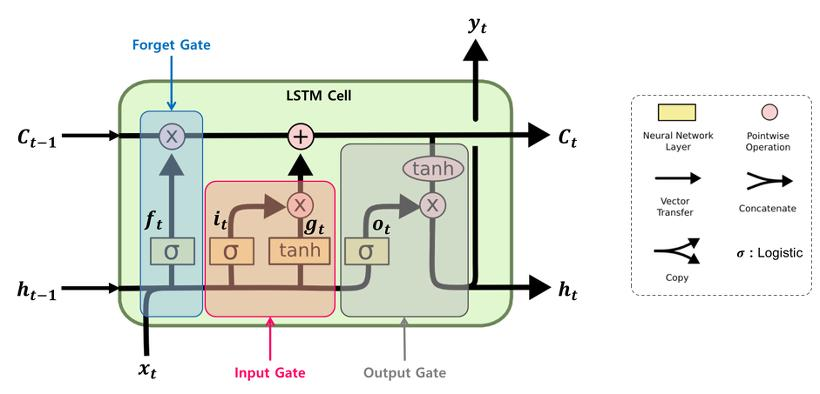
\includegraphics[width=0.4\textwidth]{Fig/LSTM.jpg}
	\caption{LSTM model structure}
\end{wrapfigure}
Compared to the traditional RNN, LSTM performs various mathematical operations, including including element-wise multiplication and addition, to control the flow of information and perform updates to the memory cell and hidden state.

Through this architecture and characteristics, LSTM can handle the long sequential data by maintaining a memory cell with gates to control information flow, 
making it capable of capturing long-term dependencies and patterns in the data.

\subsubsection{GRU}

\begin{wrapfigure}{r}{0.4\textwidth}
	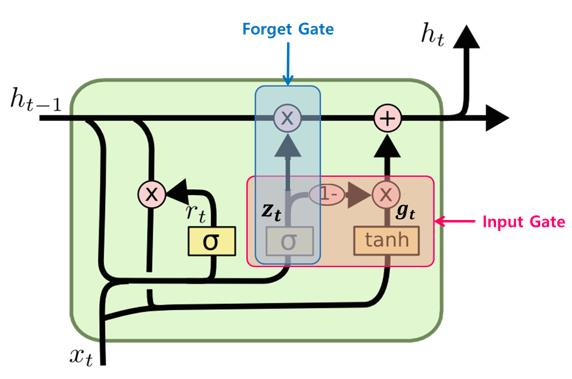
\includegraphics[width=0.4\textwidth]{Fig/GRU.jpg}
	\caption{GRU model structure}
\end{wrapfigure}
A Gated Recurrent Unit(GRU) is another type of recurrent neural network (RNN) architecture, 
similar to the Long Short-Term Memory (LSTM) network. 
GRUs are simpler in structure compared to LSTMs but have been found to be highly effective in various applications. 
GRU is also designed to address the vanishing gradient problem and enable RNNs to better capture long-range dependencies in sequential data. 
Compared to LSTM, GRU does not distinguish between cell status and the output.

GRU has two gates: reset gate and update gate.
\begin{enumerate}
	\item Reset gate: Reset gate is denoted by color box. It decides how much of the past information to forget.
	\item Update gate: Update gate is denoted by color box. It decides how much of the past information to remember.
\end{enumerate}

GRUs also perform mathematical operations, including element-wise multiplications and additions, to control the flow of information and update the hidden state.

Through this architecture and characteristics, GRU can also handle the long sequential data by maintaining a memory cell with gates to control information flow, 
making it capable of capturing long-term dependencies and patterns in the data.


\subsubsection{One-dimensional CNN}

\begin{wrapfigure}{r}{0.4\textwidth}
	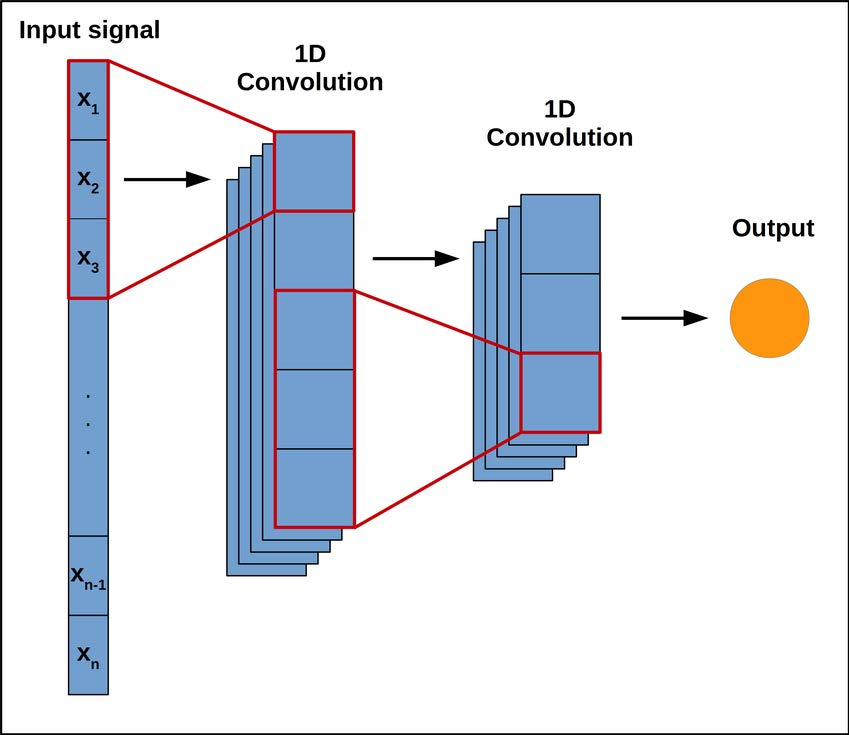
\includegraphics[width=0.4\textwidth]{Fig/CNN.jpg}
	\caption{CNN model structure}
\end{wrapfigure}
A Convolutional Neural Network(CNN) is a neural network architecture widely employed for processing and analyzing one-dimensional data sequences. 
In the context of stock price prediction, which inherently involves one-dimensional data, the utilization of a one-dimensional CNN is particularly relevant and effective.

Compared to other recurrent neural network (RNN) variants like LSTM and GRU, CNNs offer a notably simpler structural design. 
Also it seems possible to analyse the various patterns of stock price data through the convolutional layers.
As the stock price data is characterized by its non-stationary nature, exhibiting evolving trends and patterns over time, 
it is probable that CNN excels the performance of LSTM, and GRU.

\subsubsection{Transformer}

\begin{wrapfigure}{r}{0.4\textwidth}
	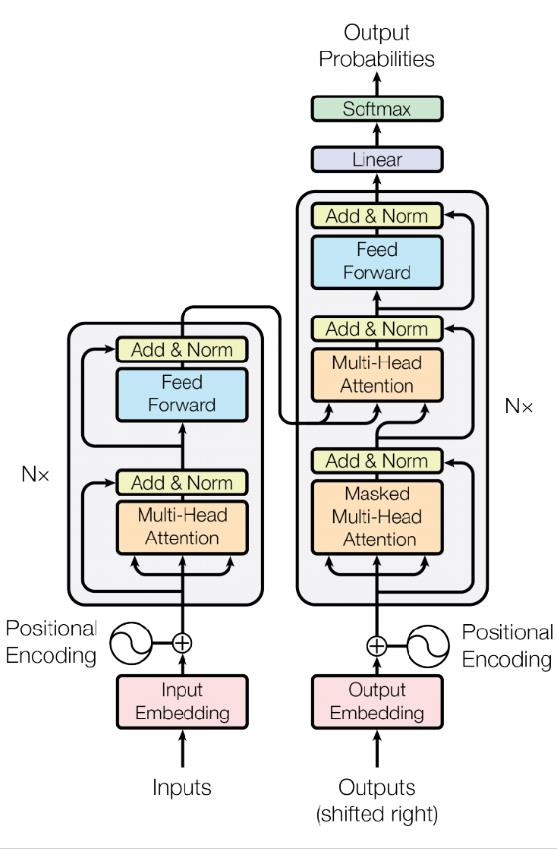
\includegraphics[width=0.4\textwidth]{Fig/Transformer.jpg}
	\caption{Transformer model structure}
\end{wrapfigure}
The Transformer is a neural network architecture that has gained significant prominence in natural language processing (NLP) tasks 
due to its remarkable effectiveness. Transformers have exhibited promising potential in the domain of time series prediction.

Transformer operates as an Encoder-Decoder model, leveraging an attention mechanism.
In the Encoder-Decoder architecture, the Encoder takes an input sequence and encodes the information into a single context vector. 
Conversely, the Decoder utilizes this context vector to generate an output sequence.
Within the model structure, a crucial component is the "embedding" process. 
This process involves the conversion of input values into a unified vector representation.

The attention mechanism employed by the Transformer is a key feature. 
It assigns varying weights to elements within the input sequence, placing greater emphasis on pertinent information. 
This emphasis is then reflected in the model's output. 
The Transformer employs this mechanism to comprehensively evaluate the significance of the entire input sequence when generating the output.

The utilization of the Transformer model holds the promise of delivering superior performance. 
It has the capacity to incorporate diverse sources of information such as news, stock indices, and corporate disclosures, distinguishing it from other models.
